\documentclass{article}
\usepackage{graphicx} % Required for inserting images
\newtheorem{problem}{Problem}
\usepackage{amssymb}
\usepackage{amsfonts}
\usepackage{amsmath}
\usepackage{tikz}

\newcommand{\parallelsum}{\mathbin{\!/\mkern-5mu/\!}}




\title{Math1810c Homework 5}
\author{Released October 10}
\date{Due October 17}

\begin{document}

\maketitle

\section{Instructions}

For the homework, you must write your own solutions for the Mathematical Problems. For the coding problems, you will work in your teams, and should have a commit on your Github page for the tasks for each week. 

\section{Mathematical Problems}

\begin{problem}
    Give a proof of Pappus's theorem when DE is parallel to BC and AB is parallel to EF. (Below is a diagram where the opposite sides of the hexagon ABCDEF are colored with the same color. 

\begin{center}
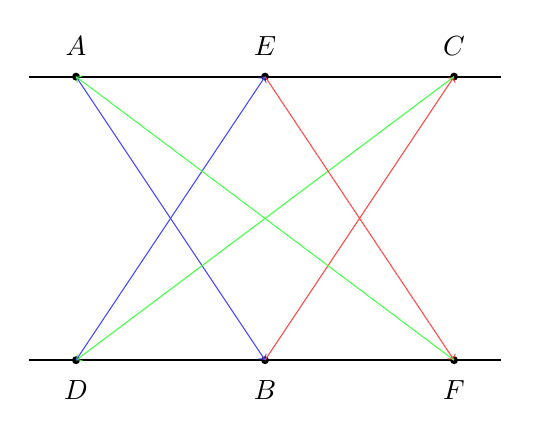
\begin{tikzpicture}[scale=1.2]
  % Base points on two parallel lines
  \coordinate (D) at (0,0);
  \coordinate (B) at (2,0);
  \coordinate (F) at (4,0);

  % Match x-coordinates on the upper line: F_x=A_x, E_x=B_x, D_x=C_x
  \coordinate (A) at (0,3);
  \coordinate (E) at (2,3);
  \coordinate (C) at (4,3);
  % Base lines
  \draw[thick] (-0.5,0) -- (4.5,0) node[below right] { };
  \draw[thick] (-0.5,3) -- (4.5,3) node[above right] { };

  % Labels
  \foreach \P/\pos in {D/below,B/below,F/below}
    \fill (\P) circle(1.2pt) node[\pos=4pt] {$\P$};
  \foreach \P/\pos in {A/above,E/above,C/above}
    \fill (\P) circle(1.2pt) node[\pos=4pt] {$\P$};

      \draw[blue!70,->,opacity=1] (A) -- (B);
      \draw[red!70,->,opacity=1] (B) -- (C);
      \draw[green!70,->,opacity=1] (C) -- (D);
      \draw[blue!70,->,opacity=1] (D) -- (E);
      \draw[red!70,->,opacity=1] (E) -- (F);
      \draw[green!70,->,opacity=1] (F) -- (A);
\end{tikzpicture}
\end{center}
\end{problem}

\begin{problem}
    Assume that you can construct an $n$-gon using a straight-edge and compass, prove that you can then construct a $2n$-gon.
\end{problem}

\begin{problem}
    Prove that the composition of two rotations of a sphere is another rotation of the sphere. 
\end{problem}

\begin{problem}
    Which of Euclid's postulates fails on the sphere, and why?
\end{problem}

\newpage

\section{Coding Goals}

\begin{problem}
    We are now going to start thinking about ``adding rabbits'' in to our system. However, we shall do this manually. If you recall in the proof of showing that three medians of a triangle are concurrent, an additional point needed to be constructed for the proof. Try to get your system to solve this problem, but have it so that you manually add the ``rabbit'' needed to solve the problem after say 5 iterations of ddar. 
\end{problem}

\begin{problem}
    Try to come up with additional problems where you might need different kinds of ``rabbits'' to solve them, and classify the problems based off of the rabbits needed to solve them. Make sure that your file construction.py can be used to generate these rabbits, and see if your system can solve these problems when given the rabbits. 
\end{problem}

\begin{problem}[Extra Credit]
    Try to implement area into your system (this may be harder), and have your system give a proof of the Pythagorean theorem. 
\end{problem}

\end{document}
